\documentclass{article}%
\usepackage[T1]{fontenc}%
\usepackage[utf8]{inputenc}%
\usepackage{lmodern}%
\usepackage{textcomp}%
\usepackage{lastpage}%
\usepackage{graphicx}%
%
\title{Ejemplo Completo de Documento en LaTeX}%
\author{Andres Tenllado Perez}%
\date{\today}%
%
\begin{document}%
\normalsize%
\maketitle%
\section{Introducción}%
\label{sec:Introduccin}%
Este documento es un ejemplo más completo de cómo generar archivos en LaTeX desde Python usando la librería pylatex.\newline%
%
Podemos incluir texto con formato como %
\textbf{negrita}%
, %
\textit{itálica}%
 y listas:\newline%
%
\begin{itemize}%
\item Primer punto de la lista%
\item Segundo punto importante%
\item Tercer punto final%
\end{itemize}

%
\section{Ecuaciones Matemáticas}%
\label{sec:EcuacionesMatemticas}%
Podemos incluir ecuaciones matemáticas en LaTeX, por ejemplo, la famosa ecuación de Einstein:%
\begin{equation} E = mc^2 \end{equation}

%
\section{Tablas}%
\label{sec:Tablas}%
Aquí hay una tabla de ejemplo:\newline%
%
\begin{tabular}{c c c}%
\hline%
Columna 1&Columna 2&Columna 3\\%
\hline%
A&B&C\\%
D&E&F\\%
\hline%
\end{tabular}

%
\section{Imágenes}%
\label{sec:Imgenes}%
También podemos agregar imágenes en LaTeX. Asegúrate de que el archivo de imagen exista en el mismo directorio.\newline%
%


\begin{figure}[h!]%
\centering%
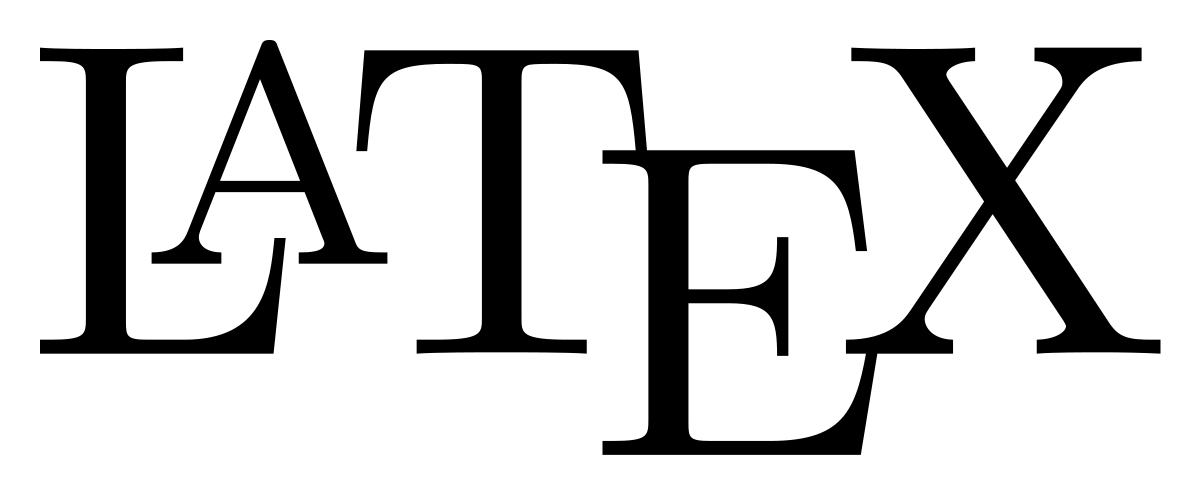
\includegraphics[width=0.5\textwidth]{latex.png}%
\caption{Ejemplo de una imagen en LaTeX.}%
\end{figure}

%
\section{Conclusión}%
\label{sec:Conclusin}%
Este ejemplo muestra cómo generar documentos en LaTeX con Python incluyendo texto con formato, ecuaciones, tablas e imágenes.

%
\end{document}